\documentclass[11pt,a4paper]{article}
\usepackage[utf8]{inputenc}
\usepackage[english]{babel}
\usepackage{graphicx}
\usepackage{multicol}
\usepackage{amsmath}
\usepackage{hyperref}
\usepackage{amsthm}
\theoremstyle{definition}
\newtheorem{definition}{Definition}
\newtheorem{ex}{Example}
\setlength{\columnsep}{1cm}


\begin{document}
\author{\textbf{Ibrahim Abou Elenein}}
\title{\textbf{Fourier Series of CT signals}}
\date {\today}
\maketitle

\textbf{Fourier series} states that, any periodic signal can 
be expressed as summation of sines and cosines 
with one fundamental frequency and infinite number

\section{Fourier Series Representation of CT Periodic Signals}
The exponential form of Fourier series (complex 
representation of continuous time periodic signals) 
\[
    \displaystyle  x(t) = \sum_{k=-\infty}^{\infty} a_k 
    e^{jk\omega_ot}
\]
Whrere: \\
$a_k$ Fourier coefficients.\\
$x(t)$ is periodic with Period $T$ whrere $\omega_o 
= \dfrac{2\pi}{T}$
\[
    x(t) = \dots + a_{-2}e^{-j2\omega_ot}
    + a_{-1}e^{-j\omega_ot} + a_o + a_{1}e^{+j\omega_ot} + \dots
\]

\subsection{Notes}
\begin{itemize}
    \item The term $a_o$ is constant (Dc coefficient)
    \item The terms $a_1  \ \& \  a_{-1}$ both have the fundemntal frequency
        as $\omega_o$ and called \textbf{first harmonic component}
    \item The terms $a_2  \ \& \  a_{0}$ both have the fundemntal frequency
        as $\omega_o$ and called \textbf{seconed harmonic component}
    \item Generalally, The components for $k=-N \ \& \ N$ are called 
        \textbf{Nth order Component}.

\end{itemize}
\section{Obtaining the Fourier Series Coefficients $a_k$}
\[
    \displaystyle x(t) = \sum_{k=-\infty}^{\infty} a_k e^{jk\omega_ot} 
\]
\[
    \displaystyle x(t)e^{-jn\omega_ot} = \sum_{k=-\infty}^{\infty} a_k e^{j(k-n)\omega_ot} \
    \text{integrating over the period}
\]
\[
    \displaystyle \int_0^T x(t)e^{-jn\omega_ot} dt =
    \int_0^T\sum_{k=-\infty}^{\infty} a_k e^{j(k-n)\omega_ot} dt \   a_k 
    \ \text{are time-independent}
\]
\[
    \displaystyle \int_0^T x(t)e^{-jn\omega_ot} dt =
    \sum_{k=-\infty}^{\infty} a_k \int_0^T e^{j(k-n)\omega_ot} dt 
\]
\[
    \displaystyle  \int_0^T e^{j(k-n)\omega_ot} dt = 
    \begin{cases}
        T, & k =n \\
        0, & k \neq n
    \end{cases} \ \text{Integration over one period of cos and sin}
\]

\[
    \underbrace{a_n = \dfrac{1}{T} \int_0^T x(t)e^{-jn\omega_ot} dt }_{\text{Fourier Series Coefficients}}
\]

\section{Fourier series of Periodic CT signal}

\[
    \displaystyle x(t) = \sum_{k=-\infty}^{\infty} a_k e^{jk\omega_ot}
\]
\[
    a_k = \dfrac{1}{T} \int_0^T x(t)e^{-jk\omega_ot} dt \ , \ \omega_o
    = \dfrac{2\pi}{T}
\]
\subsection{Constant Value}
This the average of $x(t)$ over one period.
\[
    a_o = \dfrac{1}{T} \int_T x(t) dt \Rightarrow \text{The area under the curve over one period }
\]
\[
    a_o = \dfrac{\text{Area of one period}}{T}
\]
\section{Famous Signals}
\subsection{DC Signal}
\[
    x(t) = A
\]
\[
    x(t) = \dots + a_{-2}e^{-j2\omega_ot}
    + a_{-1}e^{-j\omega_ot} + a_o + a_{1}e^{+j\omega_ot} + \dots
\]
So by comparing 

\[
    \boxed{\ a_o = A \ \ \& \ \  a_k = 0 \ \text{for} \ k \neq 0}
\]
\subsection{Complex Exponential}
\[
    x(t) = e^{j\omega_ot}
\]
\[
    x(t) = \dots + a_{-2}e^{-j2\omega_ot}
    + a_{-1}e^{-j\omega_ot} + a_o + a_{1}e^{+j\omega_ot} + \dots
\]
So by comparing 
\[
    \boxed{a_1 = 1 \ \ \& \ \ a_k = 0  \ \text{for} \  k \neq 1}
\]
Note if 
\[
    x(t) = 2e^{-3j\omega_ot} \Rightarrow a_{-3} = 2 \ \ \& \ \ a_k = 0  \ \text{for} \ k \neq -3
\]
\subsection{Sinusoidals}
\subsubsection{Cosine}
\[
    x(t) = \cos(\omega_ot) = \underbrace{\dfrac{1}{2} e^{j\omega_ot} + \dfrac{1}{2} e^{-j\omega_ot}}_{\text{Euler's rule}}
\]
\[
    x(t) = \dots + a_{-2}e^{-j2\omega_ot}
    + a_{-1}e^{-j\omega_ot} + a_o + a_{1}e^{+j\omega_ot} + \dots
\]
So by comparing 
\[
    \boxed{a_1 = a_{-1} = \frac{1}{2} \ \ \& \ \ a_k = 0  \ \
    \text{for} \ \ k \neq 1, -1 }
\]
\subsubsection{Sine}
\[
    x(t) = \sin(\omega_ot) = \underbrace{\dfrac{1}{2j} e^{j\omega_ot} + \dfrac{-1}{2j} e^{-j\omega_ot}}_{\text{Euler's rule}}
\]
\[
    x(t) = \dots + a_{-2}e^{-j2\omega_ot}
    + a_{-1}e^{-j\omega_ot} + a_o + a_{1}e^{+j\omega_ot} + \dots
\]
So by comparing 
\[
    \boxed{a_1 = \frac{1}{2j},a_{-1} =\frac{-1}{2j}  \ \ \& \ \ a_k = 0  \ \
    \text{for} \ \ k \neq 1, -1 }
\]
\subsubsection{Example}
Find Fourier Series representation of the following Signal 

\[
    x(t) = 1 + \sin(\omega_ot) + 2 \cos(\omega_ot) + \cos(2\omega_ot + \frac{\pi}{4})
\]
\[
    x(t) = 1 + \frac{1}{2j}[e^{j\omega_ot}-e^{-j\omega_ot}] + 
    [e^{j\omega_ot} + e^{-j\omega_ot}] + \frac{1}{2} [e^{j(2\omega_ot+\frac{\pi}{4})} 
    + e^{-j((2\omega_ot+\frac{\pi}{4}))}] = 
\]
Collecting like terms
\[
    x(t) = 1 + (1 + \frac{1}{2j}) e^{j\omega_ot} +(1 - \frac{1}{2j}) e^{-j\omega_ot} 
    + (\frac{1}{2} e^{j\frac{\pi}{4}}) e^{j2\omega_ot} + (\frac{1}{2} e^{-j\frac{\pi}{4}}) e^{-j2\omega_ot}
\]
\[
    x(t) = \underbrace{1}_{a_0} + \overbrace{(1 + \frac{1}{2j})}^{a_1} e^{j\omega_ot} 
    + \underbrace{(1 - \frac{1}{2j})}_{a_{-1}} e^{-j\omega_ot} 
    + \overbrace{(\frac{1}{2} e^{j\frac{\pi}{4}})}^{a_2} e^{j2\omega_ot} +
    \underbrace{(\frac{1}{2} e^{-j\frac{\pi}{4}})}_{a_{-2}} e^{-j2\omega_ot}
\]
\[
    a_0 = 1, \ \ a_1 = (1+\frac{1}{2j}), \ \ a_{-1} = (1-\frac{1}{2j}),  \ \ 
    a_2 = \frac{1}{2} e^{j\frac{\pi}{4}}, \ \ a_2 = \frac{1}{2} e^{-j\frac{\pi}{4}},
    \ \ a_k = 0 \ \ \text{for} \ |k| > 2 
\]
\subsection{Periodic Impulse Train}
Unit Impulse $(\delta(t))$ repating itself every period T 
\begin{center}
    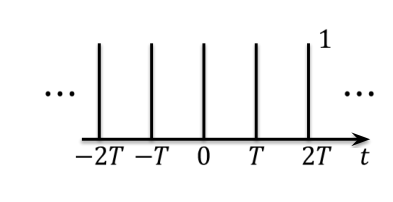
\includegraphics[width=201px]{impulse-train.png}

\end{center}
\[
    \boxed{a_k = \frac{1}{T}}
\]
\textbf{Note} The periodic impulse train must be centered at 0 and has amplitude $=1$
Otherwise, it will be a shifted and scaled periodic impulse train.
\end{document}
